% !TEX root = RJwrapper.tex
\title{\pkg{rotations}: An R Package for $SO(3)$ Data}
\author{by Bryan Stanfill, Heike Hofmann, Ulrike Genschel}

\maketitle

\abstract{
In this article we introduce the \pkg{rotations} package which provides users with the ability to simulate, analyze and visualize three-dimensional rotation data.  More specifically it includes four commonly used distributions from which to simulate data, five estimators of the central orientation, seven confidence region estimation procedures and a novel approach to visualizing these data.  All of the above features are available to two different parameterizations of rotations: three-by-three matrices and quaternions.  In addition two datasets are included that illustrate the use of rotation data in practice.
}

\section{Introduction}

Data in the form of three-dimensional rotations find application in many scientific areas, such as bio-medical engineering, computer vision, and geological and materials sciences where such data represent the positions of objects within some three-dimensional reference frame.  For example, \cite{humbert1996, bingham2009, bachmann2010} apply rotation data to study the orientation of cubic crystals on the surfaces of metal.  \cite{rancourt2000} use rotations to represent  variations in human movement while performing a task. 

A common goal shared in the analysis of this kind of data across all these fields is to estimate the main or central orientation for a sample of rotations. 
More formally, let  $SO(3)$ denote the  rotation group, which consists of all real-valued $3\times 3$  matrices $R$ with determinant equal to +1.
Then observations $\bm{R}_1,\ldots,\bm{R}_n \in SO(3)$ can be conceptualized as a random sample from a \textit{location model}
\begin{equation}
\label{eqn:loc_model}
\mathbf{R}_i = \bm{S} \bm{E}_i, \quad i=1,\ldots,n,
\end{equation}
where $\bm S \in SO(3)$ is the {\it fixed} parameter of interest indicating the central orientation, and $\bm{E}_1,\ldots,\bm{E}_n \in SO(3)$ denote i.i.d. {\it random} rotations which symmetrically perturb $\bm{S}$.  Model \eqref{eqn:loc_model} is a rotation-matrix analog of a location model for scalar data $Y_i = \mu + e_i$, where $\mu \in \mathbb{R}$ denotes a mean and $e_i \in \mathbb{R}$ denotes an additive error symmetrically distributed around zero.

While there is a multitude of packages and functions available in R to estimate the mean in a location model; the toolbox for rotational data is limited.  The \CRANpkg{orientlib} \citep{murdoch2003} package includes the definition of an orientation class along with a few methods to summarize and visualize rotation data.  A strength of the \pkg{orientlib} package is its thorough exploration of rotation representations, but the estimation and visualization techniques are lacking and no methods for inference are available.  The \CRANpkg{onion} package includes functions for rotation algebra but only the quaternion form is available and data analysis is not possible  \citep{hankin2011}.  The \pkg{uarsbayes}  \citep{qu2013} package includes functions for data generation and Bayes inference but this package is currently not publicly available.  Packages for circular and spherical data, e.g. \CRANpkg{circular} \citep{agostinelli2011} and \CRANpkg{SpherWave} \citep{oh2013}, can possibly be used but their extension to rotation data is not trivial or straightforward.

The \CRANpkg{rotations} package fills this void by providing users with the tools necessary to simulate rotations from \eqref{eqn:loc_model} allowing for several distributions for the perturbation matrices $\bm E_i$.  Estimation and inference for $\bm{S}$ in \eqref{eqn:loc_model} from both frequentist and Bayesian perspectives are available along with novel visualization techniques.  The remainder of this manuscript introduces rotation data more fully and discusses the ways they are handled by Version 1.0 of the \pkg{rotations} package.

\section{Rotation parameterizations}

Several parameterizations of rotations exist. We consider two of the most commonly used: orthogonal $3\times 3$ matrices with determinant one and four-dimensional unit vectors called \dfn{quaternions}.  The \pkg{rotations} package allows for both parameterizations as input as well as transforming one into the other. We will briefly discuss each:

\subsection{Matrix form}\label{subsec:matrix}

Rotations in three-dimensions can be represented by $3\times3$ orthogonal matrices with determinant one.  Matrices with these characteristics form a group called the \dfn{special orthogonal group}, or \dfn{rotation group}, denoted $SO(3)$.  Every element in $SO(3)$ is associated with a skew-symmetric matrix $\Phi(\bm W)$ where
\[
\bm{\Phi}(\bm{W}) = \left(\begin{array}{ccc}0 & -w_3 & w_2 \\ w_3 & 0 & -w_1 \\-w_2 & w_1 & 0\end{array}\right)
\]
and $\bm W\in\mathbb{R}^3$.  Applying the exponential operator to the matrix $\Phi(\bm W)$ results in the rotation $\bm R$
\begin{equation}\label{eqn:expW}
  \bm R=\exp[\bm{\Phi}(\bm{W})] = \sum\limits_{k=0}^\infty \frac{[\bm{\Phi}(\bm{W})]^k}{k!}.
  \end{equation}
Since $\bm\Phi(\bm W)$ is skew-symmetric, it can be show that \eqref{eqn:expW} reduces to
\begin{equation}\label{eqn:angleAxis}
\bm R =\cos(r)\bm{I}_{3\times3} + \sin(r) \bm{\Phi}(\bm{U}) + [1-\cos (r)] \bm{U} \bm{U}^\top
\end{equation}
where $r=\|\bm{W}\|$, $\bm{U} =\bm{W}/\|\bm{W}\|$.  In the material sciences literature the values $r$ and  $\bm U\in\Rbb^3$ are termed the \dfn{misorientation angle} and \dfn{misorientation axis}, respectively.

Given a rotation matrix $\bm R$ one can find the associated skew-symmetric matrix $\bm{\Phi}(\bm W)$ by applying the logarithm operator defined by
\begin{equation}\label{eqn:matLog}
\Log(\bm R)=\begin{cases}
\bm 0 &\text{if } \theta=0\\
\frac{r}{2\sin r}(\bm R-\bm R^\top)&\text{otherwise}
\end{cases}
\end{equation}
where $r\in[-\pi,\pi)$ satisfies $\tr(\bm R)=1+2\cos r$.  For more on the correspondence between $SO(3)$ and skew-symmetric matrices see \cite{stanfill2013}.

The \pkg{rotations} package defines the \code{S3} class \code{"SO3"}, which internally stores a sample of $n$ rotations as a $n\times9$ matrix.  If $n=1$ then an object of class \code{"SO3"} is printed as a $3\times3$ matrix but for $n>1$ the $n\times9$ matrix is printed.  Objects can be coerced into, or tested for the class \code{"SO3"} with the \code{as.SO3} and \code{is.SO3} functions, respectively.  Any object passed to \code{is.SO3} is tested for three characteristics: dimensionality, i.e. is $n\times 9$ for some integer $n$, orthogonality and determinant one.

The \code{as.SO3} function coerces the input into the class \code{"SO3"}.  Given an angle $r$ and axis $\bm U$, \code{as.SO3} will form a matrix according to \eqref{eqn:angleAxis}; given a three-dimensional vector $\bm W$ the length of that vector will be taken to be the angle of rotation $r=\|\bm W\|$ and the axis is taken to be the unit-vector in the direction of $\bm W$, $\bm U=\bm W/\|\bm W\|$.  Alternatively, one can also supply a rotation $\bm Q$ in the quaternion representation then the \code{as.SO3} function returns the matrix equivalent of $\bm Q$.  For all input types the function \code{as.SO3} returns an $n\times9$ matrix of class \code{"SO3"} where each row corresponds to a rotation matrix.    Below we illustrate the use of the \code{as.SO3} function by constructing first the $3\times3$ matrix associated with a $90^\circ$ rotation about the $y$-axis, i.e. $r=\pi/2$ and $\bm U=(0,1,0)$, rounded to three digits.

\begin{example}
> r <- pi/2
> U <- c(0, 1 ,0)
> W <- U*r
> R <- as.SO3(W)
> R
     [,1] [,2] [,3]
[1,]    0    0    1
[2,]    0    1    0
[3,]   -1    0    0
> identical(R, as.SO3(U, r))
[1] TRUE
\end{example}

Given a rotation matrix $\bm R$, the functions \code{mis.angle} and \code{mis.axis} will determine the misorientation angle and axis of an object with class \code{"SO3"} as illustrated in the next example. 
\begin{example}
> mis.angle(R)*2/pi
1
> mis.axis(R)
[1] 0 1 0
\end{example}

\subsection{Quaternion form}

Quaternions are unit vectors in $\mathbb{R}^4$ that can be expressed as the sum of one real entry and three imaginary parts
\begin{equation}\label{eqn:quat}
\bm Q = x_1 + x_2 i + x_3 j + x_4 k
\end{equation}
where $i^2 = j^2= k^2 =ijk= -1$.  We can write $\bm Q=(s,\bm V)$ as tuple of the scalar $s$ for coefficient $\bm 1$ and vector $\bm V$ for the imaginary coefficients, i.e. $s=x_1$ and $\bm V= (x_2, x_3, x_4)$.

A rotation around axis $\bm U$ by angle $r$ translates to $\bm Q=(s,\bm V)$ with
\[
s = \cos{(r/2)},  \ \ \bm V = \bm U \sin {(r/2)}.
\]
Note that rotations in quaternion form are over-parametrized: $\bm Q$ and $-\bm Q$ represent equivalent rotations.  This ambiguity has no impact on the distributional models, parameter estimation or inference methods to follow.  Hence, for consistency, the \pkg{rotations} package only generates quaternions satisfying $x_1\geq0$.  Data provided by the user does not need to satisfy this condition, however.


The \code{S3} class \code{"Q4"} is defined to manipulate rotations of this parameterization with all the same functionality available for the class \code{"SO3"}, e.g. \code{is.Q4} and \code{as.Q4} will test for, and if necessary, coerce to  class \code{"Q4"}.  Internally, a sample of $n$ quaternions is stored  in form of  a $n\times4$ matrix with each row a unit vector. Single quaternions are printed according to the representation in \eqref{eqn:quat} (see example below) while a sample of size $n$ is printed as a $n\times 4$ matrix with column names \code{Real}, \code{i}, \code{j} and \code{k} to distinguish between the real and complex components.

The following code creates the same rotation from the previous section in the form of a quaternion with the \code{as.Q4} function.  This function works much the same way as the \code{as.SO3} function in terms of possible inputs but returns a vector of length four of the class \code{"Q4"}.   We round the output to three digits for compactness.

\begin{example}
> as.Q4(U, r)
0.707 + 0 * i + 0.707 * j + 0 * k
> as.Q4(as.SO3(U, r))
0.707 + 0 * i + 0.707 * j + 0 * k
\end{example}

\section{Data generation\label{section:generation}} 

If the rotation $\bm{E}_i\in SO(3)$ from \eqref{eqn:loc_model} has an axis $\bm U$ that is uniformly distributed on the unit sphere and an angle $r$ that is independently distributed about $0$ according to some symmetric distribution function then $\bm E_i$ is said to belong to the \dfn{uniform-axis random spin}, or \dfn{UARS}, class of distributions.   From \cite{bingham2009} the density for $\bm E_i$ is given by
\begin{equation*}%\label{eq:uarsden}
f(\bm E_i|\kappa)=\frac{4\pi}{3-\tr(\bm E_i)}C\left(\left.\text{acos}\left\{[\tr(\bm E_i)-1]/2\right\}\right|\kappa\right)
\end{equation*}
where $C(\cdot|\kappa)$ is the distribution function connected to the angle of rotation $r$ with concentration parameter $\kappa$.  Members of the UARS family of distributions are differentiated based on the angular distribution.

The \pkg{rotations} package allows the user access to four members of the UARS class.  Each member is differentiated by the distribution function for $r$: the uniform distribution on the circle, the matrix Fisher \citep{langevin2005, downs1972, khatri1977, jupp1979}, the Cayley  \citep{Schaeben1997, leon2006} and a circular-von Mises-based distribution \citep{bingham2009}.  The uniform distribution on the sphere also plays the role of a uniform measure for $SO(3)$ called the Haar measure.  

The spread of  the Cayley, matrix Fisher and circular-von Mises distributions is controlled by the concentration parameter $\kappa$.  Note that concentration is a distribution specific parameter and not compatible across different distributions.  To make comparisons across distribution possible we also allow for specification of the circular variance, which is defined as $\nu=1-E[\cos(r)]$ where $E[\cos(r)]$ is often referred to as the \dfn{mean resultant length} \citep{fisher1996book}.    The form of each angular distribution along with the circular variance as a function of the concentration parameter is given in Table \ref{tab:Crforms}.


\begin{table}[h!]
\centering
\small{
\begin{tabular}{ lcccccl}\toprule
\textbf{Name}  & & \textbf{Density} $C(r |\kappa)$ & & \textbf{Circular variance $\nu$}& & \textbf{Function}\\ \midrule 
Uniform  & & $\frac{1-\cos(r)}{2\pi}$ & & $\frac{3}{2}$& & \code{-haar} \\

\rule[2mm]{0mm}{6mm} Cayley  & & $\frac{\Gamma(\kappa+2)(1+\cos r)^\kappa(1-\cos r)}{2^{(\kappa+1)}\sqrt{\pi}\Gamma(\kappa+1/2)}$ & & $\frac{3}
{\kappa+2}$ & & \code{-cayley}\\

\rule[2mm]{0mm}{6mm} matrix Fisher  & & $\frac{[1-\cos(r)]\exp[2\kappa 
\cos(r)]}{2\pi[\mathrm{I_0}(2\kappa)-\mathrm{I_1}(2\kappa)]}$ & & 
$\frac{3\mathrm{I}_0(2\kappa)-4\mathrm{I}_1(2\kappa)+\mathrm{I}_2(2\kappa)}
{2[\mathrm{I}_0(2\kappa)-\mathrm{I}_1(2\kappa)]}$& & \code{-fisher} \\

\rule[2mm]{0mm}{6mm} circular-von Mises  & & $\frac{\exp[\kappa\cos(r)]}{2\pi \mathrm{I_0}(\kappa)}$&  & 
$\frac{\mathrm{I_0}(\kappa)-\mathrm{I_1}(\kappa)}{\mathrm{I_0}(\kappa)}$& & \code{-vmises} \\[-7mm] 
\rule[2mm]{0mm}{6mm} & & & & & & \\\bottomrule
\end{tabular}}
\caption{Circular densities with respect to the Lebesgue measure and circular variance $\nu$; $I_i(\cdot)$ represents the modified Bessel function of order $i$ and $\Gamma(\cdot)$ is the gamma function.}  \label{tab:Crforms}
\end{table}


For a given concentration \code{d}, \code{p} and \code{r} take the same meaning as for the more familiar distributions such as \code{dnorm}.  To simulate a sample of $SO(3)$ data, the \code{ruars} function takes arguments \code{n}, \code{rangle}, and \code{kappa} to specify the sample size, angular distribution and concentration as shown below.  Alternatively, one can specify the circular variance $\nu$.  Note: circular variance takes precedence over  concentration in case both are provided.  The \code{space} argument determines the parameterization to form.   Note that if a single rotation is printed, then the rotation is printed as a $3\times3$ matrix as demonstrated in Section \ref{subsec:matrix}. If a sample of rotations is printed then the $n\times 9$ matrix is printed along with column titles that specify which element of the matrix each row corresponds to.  For example, the $\bm R_{\{1,1\}}$ element of a rotation matrix is printed under the column heading \code{R11} as illustrated below.   Note that we rounded the output to three digits for compactness.

\begin{example}
> Rs <- ruars(n = 20, rangle = rcayley, kappa = 1, space = 'SO3')
> Qs <- ruars(n = 20, rangle = rcayley, kappa = 1, space = 'Q4')
> Rs <- ruars(n = 20, rangle = rcayley, nu = 1, space = 'SO3')
> Qs <- ruars(n = 20, rangle = rcayley, nu = 1, space = 'Q4')
> head(Rs,3)
         R11    R21   R31   R12    R22    R32    R13     R23   R33
[1,] -0.4253 -0.850 0.310 0.475 -0.501 -0.723  0.770 -0.1602 0.617
[2,] -0.5645 -0.733 0.379 0.745 -0.256  0.615 -0.354  0.6299 0.691
[3,]  0.0874 -0.716 0.692 0.117  0.698  0.707 -0.989  0.0193 0.145
\end{example}

\section{Data analysis\label{section:analysis}}

In this section we present functions in the \pkg{rotations} package to compute point estimates and confidence regions for the central orientation $\bm S$.

\subsection{Estimation of central orientation}

Given a sample of $n$ observations $\bm R_1,\dots,\bm R_{n}$ generated according to \eqref{eqn:loc_model} the \pkg{rotations} package offers four  built-in ways to estimate the central orientation $\bm S$ from a frequentest perspective.  These estimators are either Riemannian- or Euclidean-based in geometry and either using the $L_2$ or $L_1$ norm, i.e.~mean- or median-type.  We briefly discuss how the choice of geometry affects estimation of $\bm S$.

The choice of geometry results in two different metrics to measure the distance between rotation matrices $\bm{R}_1$ and $\bm{R}_2 \in SO(3)$. The Euclidean distance, $\Edist$, between two rotations is defined by
\begin{equation*}
%\label{d_E}
\Edist(\bm{R}_1,\bm{R}_2)=\|\bm{R}_1-\bm{R}_2\|_F
\end{equation*}
where $\|\bm{A}\|_F = \sqrt{\mathbf{tr}({\bm A^\top \bm A})}$ denotes the Frobenius norm and $\mathbf{tr}(\cdot)$ denotes the trace of a matrix.  It follows $\Edist(\cdot,\cdot)$ is an extrinsic distance measure.  The Euclidean distance between two rotation matrices corresponds to the length of the shortest path in $\Rbb^{3\times3}$ that connects them.  

Estimators based on the Euclidean distance form the class of \dfn{projected} estimators.  The name is derived from the algorithms used to compute these estimators, which find the generic $3\times 3$ matrix that minimizes the loss function then projects that matrix into $SO(3)$.  For an object with class \code{"SO3"} the \code{median} or \code{mean} function with argument \code{type="projected"} will return a $3\times 3$ matrix in $SO(3)$ that minimizes the first- or second-order loss function, respectively.

By staying in the Riemannian space $SO(3)$, called the intrinsic approach, the natural distance metric becomes the Riemannian (or geodesic) distance, $\Rdist$, which for two rotations $\bm{R}_1,\bm{R}_2\in SO(3)$  is  defined as 
\begin{equation*}
%\label{d_R}
\Rdist(\bm{R}_1,\bm{R}_2)=  \frac{1}{\sqrt{2}}\|\text{Log}(\bm{R}_1^\top\bm{R}_2)\|_F = |r|,
\end{equation*}
where $\text{Log}(\bm{R})$ denotes the logarithm of $\bm{R}$ defined in \eqref{eqn:matLog} and $r\in[-\pi,\pi)$ is the misorientation angle of $\bm{R}_1^\top \bm{R}_2$.  The Riemannian distance corresponds to the length of the shortest path that connects $\bm{R}_1$ and $\bm{R}_2$ {\it within} the space $SO(3)$. For this reason, the Riemannian distance is often considered the more natural metric on $SO(3)$.  As proven in \cite{stanfill2013}, the Euclidean and Riemannian distances are related by $2\sqrt{2}\sin\left[\Rdist(\bm R_1,\bm R_2)/2\right]=\Edist(\bm R_1,\bm R_2)$.

The distance between two objects of class \code{"SO3"}, e.g. \code{R1} and \code{R2}, is computed by the function \code{rot.dist}.  The argument \code{method} specifies which type of distance to compute where the default option is \code{"extrinsic"}, which will return the Euclidean distance while setting the option to \code{"intrinsic"} will return the Riemannian.  If only one object \code{R1} is provided then the second object \code{R2} is set to the $3\times3$ identity matrix.  The input \code{R1} can an $n\times9$ matrix representing a sample of rotations, then \code{rot.dist} will return a vector of length $n$ where the $i$th element represents the specified rotational distance between the $i$th row of \code{R1} and \code{R2}.

Estimators based on the Riemannian distance metric are called \code{geometric} estimators because they preserve the geometry of $SO(3)$.  These can be computed using the \code{mean} and \code{median} functions with the argument \code{type="geometric."}  Table~\ref{tab:ests.sum} summarizes the four estimators including their formal definition and how they can be computed.  


The estimators in Table~\ref{tab:ests.sum} find estimates  based on minimization of $L_1$- and $L_2$-norms in the chosen geometry. The  function \code{gradient.search} provides the option to optimize for any other arbitrary minimization criterion. As the name suggests, the minimization is done along the gradient of the minimization function in the rotation space. Starting from an initial, user-specified rotation, the algorithm finds a (local) minimum by stepping iteratively in the direction of the steepest descent. Step size is regulated internally by adjusting for curvature of the minimization function.

We highlight this process  in the example below. The function \code{L1.error} is defined to minimize the intrinsic $L_1$-norm, the result from the optimization should therefore agree with the geometric median of the sample. In fact, the difference between the two results is at the same level as the minimal difference (\code{minerr}) used for convergence of the gradient search. What is gained in flexibility of the optimization is, of course, paid for in terms of speed: the built-in median function is faster by far than the gradient search. 

\begin{verbatim}
# error function definition
L1.error <- function(sample, Shat) {
    sum(rot.dist(sample, Shat, method = "intrinsic", p = 1))
}

cayley.sample <- ruars(n = 50, rangle = rcayley, nu = 1, space = "SO3")

# gradient based optimization
system.time(SL1 <- gradient.search(cayley.sample, L1.error))
   user  system elapsed 
  2.594   0.005   2.599 

# in-built function
system.time(S <- median(cayley.sample, type = "geometric"))
   user  system elapsed 
  0.005   0.000   0.006 
  
rot.dist(S, SL1$Shat)
[1] 1.492e-05
\end{verbatim}


\begin{table}[h]
\centering
\begin{tabular}{ lclclcl}\toprule
\rule[2mm]{0mm}{1mm} \textbf{Estimator name} & & \textbf{Definition} & & \textbf{Code}\\ 
\midrule
Projected Mean & & $\ProjMean=\underset{\bm S\in SO(3)}{\argmin}\sum\limits_{i=1}^n d_E^2(\bm S,\bm R_i)$ & & \code{mean(Rs, type = "projected")} \\
\rule[2mm]{0mm}{6mm} Projected Median & & $\ProjMedian=\underset{\bm S\in SO(3)}{\argmin}\sum\limits_{i=1}^nd_E(\bm S,\bm R_i)$ & & \code{median(Rs, type = "projected")} \\
\rule[2mm]{0mm}{6mm} Geometric Mean & & $\GeomMean=\underset{\bm S\in SO(3)}{\argmin}\sum\limits_{i=1}^n d_R^2(\bm S,\bm R_i)$&  & \code{mean(Rs, type = "geometric")} \\
\rule[2mm]{0mm}{6mm} Geometric Median & & $\GeomMedian=\underset{\bm S\in SO(3)}{\argmin}\sum\limits_{i=1}^n\Rdist(\bm S,\bm R_i)$&  & \code{median(Rs, type = "geometric")} \\[-7mm] 
\rule[2mm]{0mm}{6mm} & & & & \\ \bottomrule
\end{tabular}
\caption{A summary of the estimators included in \pkg{rotations} package.  \code{Rs} is a sample of $n$ rotations with class \code{"SO3"} or \code{"Q4"} as generated in the Section \ref{section:generation}.}  \label{tab:ests.sum}
\end{table}

\subsection{Confidence regions\label{subsec:regions}}

Asymptotic results for the distribution of the projected mean $\ProjMean$ and median $\ProjMedian$, see Table \ref{tab:ests.sum}, can be used to construct confidence regions for the central orientation $\bm S$. In the literature two approaches are taken to derive the limiting distribution of the vector that generates to the centered estimator.  More specifically, the vector $\widehat{\bm h}$ satisfying
\[
\exp[\bm{\Phi}(\widehat{\bm h})]=\bm S^\top\ProjMean
\]
has been shown to have a multivariate normal distribution.  The first employs results about matrix decompositions while the other takes a moment-based approach.  A brief summary of these methods is given next.

\cite{prentice1986} used results found in \cite{tyler1981} and the fact that $\ProjMean$ is a function of the spectral decomposition of $\overline{\bm R}=\sum_{i=1}^n\bm{R}_i/n$ in order to justify a multivariate normal limiting distribution for the scaled vector $\sqrt{n}\,\widehat{\bm h}$.  Unsatisfied with the coverage rate achieved by \cite{prentice1986}, \cite{fisher1996Boot} proposed a pivotal bootstrap procedure that results in coverage rates closer to the nominal in even small samples.  Note that $\ProjMedian$ cannot be expressed as a function of the sample spectral decomposition, therefore this approach is not applicable.

It has also been shown that both estimators $\ProjMean$ and $\ProjMedian$ are M-estimators allowing for a moment-based approach to confidence region estimation.  \cite{chang2001} used this moment-based approach to estimate a confidence region for the central orientation based on the normal limiting distribution.  In an unpublished report by Drs. Zhang and Nordman a pivotal bootstrap approach was implemented to improve coverage rates in small samples.

These six methods are available through the wrapper function \code{region}.  They are differentiated based on the \code{method}, \code{type} and \code{estimator} arguments.  Set \code{estimator="mean"} or  \code{estimator="median"} to estimate a region based on $\ProjMean$ or $\ProjMedian$, respectively.  For $\ProjMean$ one can choose \code{method="eigen"} for the eigenvector-based methods or \code{method="moment"} for the moment-based approach.  Since the eigenvector-based methods cannot be applied to $\ProjMedian$ an error is returned if \code{method="eigen"} and \code{estimator="median"} are combined.  A bootstrap version of the specified method is implemented if \code{type="bootstrap"} or the normal limiting distribution can be chosen with \code{type="theory"}.  If a bootstrap type region is specified one can additionally specify the bootstrap sample size with the \code{m} argument, which is set to 300 by default.  Regardless of the method and type chosen a single value is returned on the interval $(0,\pi]$.  This value corresponds to the radius of the confidence region centered at each of the axes of the respective estimators.  

In the example code below a sample of $n=50$ rotations are drawn from the Cayley-UARS($\bm I_{3\times 3}, \kappa=10$) distribution then the four types of moment-based confidence regions are constructed.  For a graphical representation of this dataset along with an interpretation of the confidence regions see Figure \ref{fig:regs}.

\begin{example}
> Rs <- ruars(50, rcayley, kappa = 10)
> region(Rs, method="moment", type="theory", estimator="mean", alp=0.05)
[1] 0.1891591
> region(Rs, method="moment", type="bootstrap", estimator="mean", alp=0.05, m=300)
[1] 0.2010779
> region(Rs, method="moment", type="theory", estimator="median", alp=0.05)
[1] 0.2008109
> region(Rs, method="moment", type="bootstrap", estimator="median", alp=0.05, m=300)
[1] 0.2491973
\end{example}

\subsection{Bayesian Methods}

The Bayesian point and credible region estimation functions in the \pkg{rotations} package are based on the Metropolis-Hastings within Gibbs algorithm described in \cite{bingham2009bayes} and \cite{bingham2010}.  With observations $\bm R_1,\dots,\bm R_n\in SO(3)$, tuning parameters $\phi$ and $\sigma^2$, and starting values $\bm S^0\in SO(3)$ and $\kappa^0$, a draw from the posterior distribution for $(\bm S^j,\kappa^j)$, $j=1,\dots,m$ is generated by the following.
\begin{enumerate}
\item Generate $\bm S^{j*}\sim F(\bm S^{j-1},\phi)$ as a proposal for $\bm S^j$.  
\item Compute $r_j^1=g_n(\bm S^{j*},\kappa^{j-1})/g_n(\bm S^{j-1},\kappa^{j-1})$.  
\item Generate $W_j^1\sim\text{Bernoulli}(\text{min}(1,r_j^1))$ and let $\bm S^j=W_j^1\bm S^{j*}+(1-W_j^1)\bm S^{j-1}$.
\item Generate $\log(\kappa^{j*})\sim N(\log(\kappa^{j-1}),\sigma^2)$, with $\kappa^{j*}$ as a candidate for $\kappa^j$.  
\item Compute $r_j^2=g_n(\bm S^{j},\kappa^{j*})\kappa^{j*}/g_n(\bm S^{j},\kappa^{j-1})\kappa^{j-1}$.  
\item Generate $W_j^2\sim\text{Bernoulli}(\text{min}(1,r_j^2))$ and let $\kappa^j=W_j^2\kappa^{j*}+(1-W_j^2)\kappa^{j-1}$. 
\end{enumerate}

The forms of the functions $F(\bm S,\phi)$ and  $g_n(\bm S,\kappa)$ vary with the distributional model assumed for the data as well as the priors chosen for the model parameters.  The function $F(\bm S,\phi)$ is the distribution from which proposal values for the central orientation parameter are drawn and is usually set to be the same distribution function used in the data likelihood.  The $g_n(\bm S,\kappa)$ function is the product of the posterior distributions and the likelihood; for its full form assuming non-informative priors and a circular-von Mises or matrix Fisher likelihood see \cite{bingham2009bayes} and \cite{bingham2010b}, respectively.  As these results have not appeared for the Cayley distributions then we describe it here.

For the Cayley distribution it can be show the Jeffreys prior for $\kappa$ is given by
\[
\pi(\kappa)=\sqrt{\psi'(\kappa+0.5)-\psi'(\kappa+2)}
\]
where $\psi'(x)=\partial^2\log[\Gamma(x)]/\partial x^2=\sum_{k=0}^\infty (x+k)^{-2}$ is the tri-gamma function.  A uniform prior on $SO(3)$ is placed on $\bm S$, that is $\pi(\bm S)=1$ with respect to the Haar measure for all $\bm S\in SO(3)$. It follows the posterior distribution for $\bm S$ and $\kappa$ is proportional to
\[
g_n(\bm S,\kappa)=\sqrt{\psi'(\kappa+0.5)-\psi'(\kappa+2)}\left[\frac{\pi^{1/2}\Gamma(\kappa+2)}{\Gamma(\kappa+0.5)}\right]^n\prod_{i=1}^n\left\{\frac{1}{2}+\frac{1}{4}\left[\tr(\bm S^\top\bm R_i)-1\right] \right\}^\kappa.
\]

The function \code{MCMCSO3}  implements the algorithm described above using non-informative priors for the parameters.  In particular a uniform prior on the space of rotations $SO(3)$ for $\bm S$ and Jeffreys prior for the concentration $\kappa$ are chosen. The function returns a list consisting of draws from the posterior distributions for $\bm S$ and $\kappa$ along with acceptance rates for both parameters.  The likelihood is differentiated by the \code{type} argument with possible options \code{"Cayley"}, \code{"Fisher"} or \code{"Mises"}.  Initial values for the central orientation and concentration parameters are set with the  \code{S0} and \code{kappa0} arguments.  The proposal distributions from which new proposal parameter values are drawn are controlled by the tuning parameters \code{tuneS} and \code{tuneK}.  These values correspond to the parameters $\phi$ and $\sigma$ in steps 1 and 4 of the algorithm, respectively.   Finally, \code{burn$\_$in}  determines the burn in period and \code{m} the final number of draws for each parameter.  %Because the tuning parameter for $\bm S$ is the concentration of the proposal distribution, increasing the tuning parameter \code{tuneS} will increase the acceptance rate, but the opposite is true for \code{tuneK}, that is larger values will result in a smaller acceptance rate. 

Bayesian point estimates for $\bm S$ and $\kappa$ are computed by the function \code{bayes.mean}.  In particular the posterior mode of the central orientation distribution and the posterior mean of the concentration distribution are returned.  Bayesian credible regions are available with the function \code{bayesCR}, which returns a list consisting of the mode of the posterior distribution for the central orientation as well as the radius of the $100(1-\alpha)\%$ credible region centered at the posterior mode, where $\alpha$ is user-specified.    Both \code{bayes.mean} and \code{bayesCR} require the same arguments as required by \code{MCMCSO3} with an additional argument for the $\alpha$ level of the region in \code{bayesCR}.  Alternatively, in the \code{region} function one can set \code{moment="bayes"} and \code{estimator="mean"} to produce Bayesian credible regions where the likelihood is specified with the \code{type} argument.

\section{Visualizations}

The \pkg{rotations} package offers a novel method to visualize $SO(3)$ data within the framework of the \CRANpkg{ggplot2} package \citep{wickham2009}.  Recall that rotations can be represented by orthogonal matrices meaning each axis, represented by each column, has length one and is perpendicular to the other axes.  This allows us to illustrate rotation axes separately as a point on the surface of a unit sphere.

Calling the \code{plot} function with a \code{"SO3"} object will result in a sphere that represents a column of the supplied data.  The \code{center} argument defines the center of the plot and is usually set to the identity rotation \code{id.SO3} or an estimate of the central orientation, e.g.~\code{mean(Rs, method="projected")}.  The user can specify which columns to visualize with the \code{col} argument with options $1$, $2$, and $3$ representing the $x$-, $y$- and $z$- axes, respectively.  If the data are concentrated in one part of the sphere then the \code{to$\_$range} argument can be set to \code{TRUE} and the range of the plot is set to the area of the sphere that contains the points. 

All of the four estimates of the central orientation can be plotted along with a sample of rotations. Setting the argument \code{estimates$\_$show="all"} will display all four simultaneously.  If only a few estimates are of interest then any combination of \code{"proj.mean"}, \code{"proj.median"}, \code{"geom.mean"} or \code{"geom.median"} are valid inputs.  The estimators are indicated by color and a legend is provided, see Figure \ref{fig:ests}. Finally, the \code{mean$\_$regions} and \code{median$\_$regions} options allow the user to draw a circle on the surface of the sphere representing the confidence region for that axis, centered at $\ProjMean$ and $\ProjMedian$ respectively.  If estimators are plotted along with the different regions then shapes represent the estimators and colors represent the region methods, see Figure \ref{fig:regs}.  Given the sample of rotations generated in Section \ref{subsec:regions} the example code below illustrates the \code{plot} function for objects of class \code{"SO3"}.  Figure \ref{figure:eye1} illustrates the results of these commands.

\begin{example}
> plot(Rs, center = mean(Rs), show_estimates = "all")
> plot(Rs, center = mean(Rs), show_estimates = "proj.mean", 
+ mean_regions = "all",  alp = .05)
\end{example}


\begin{figure}[h]
	\centering
	\begin{subfigure}[h]{.25\textheight}
		\centering
		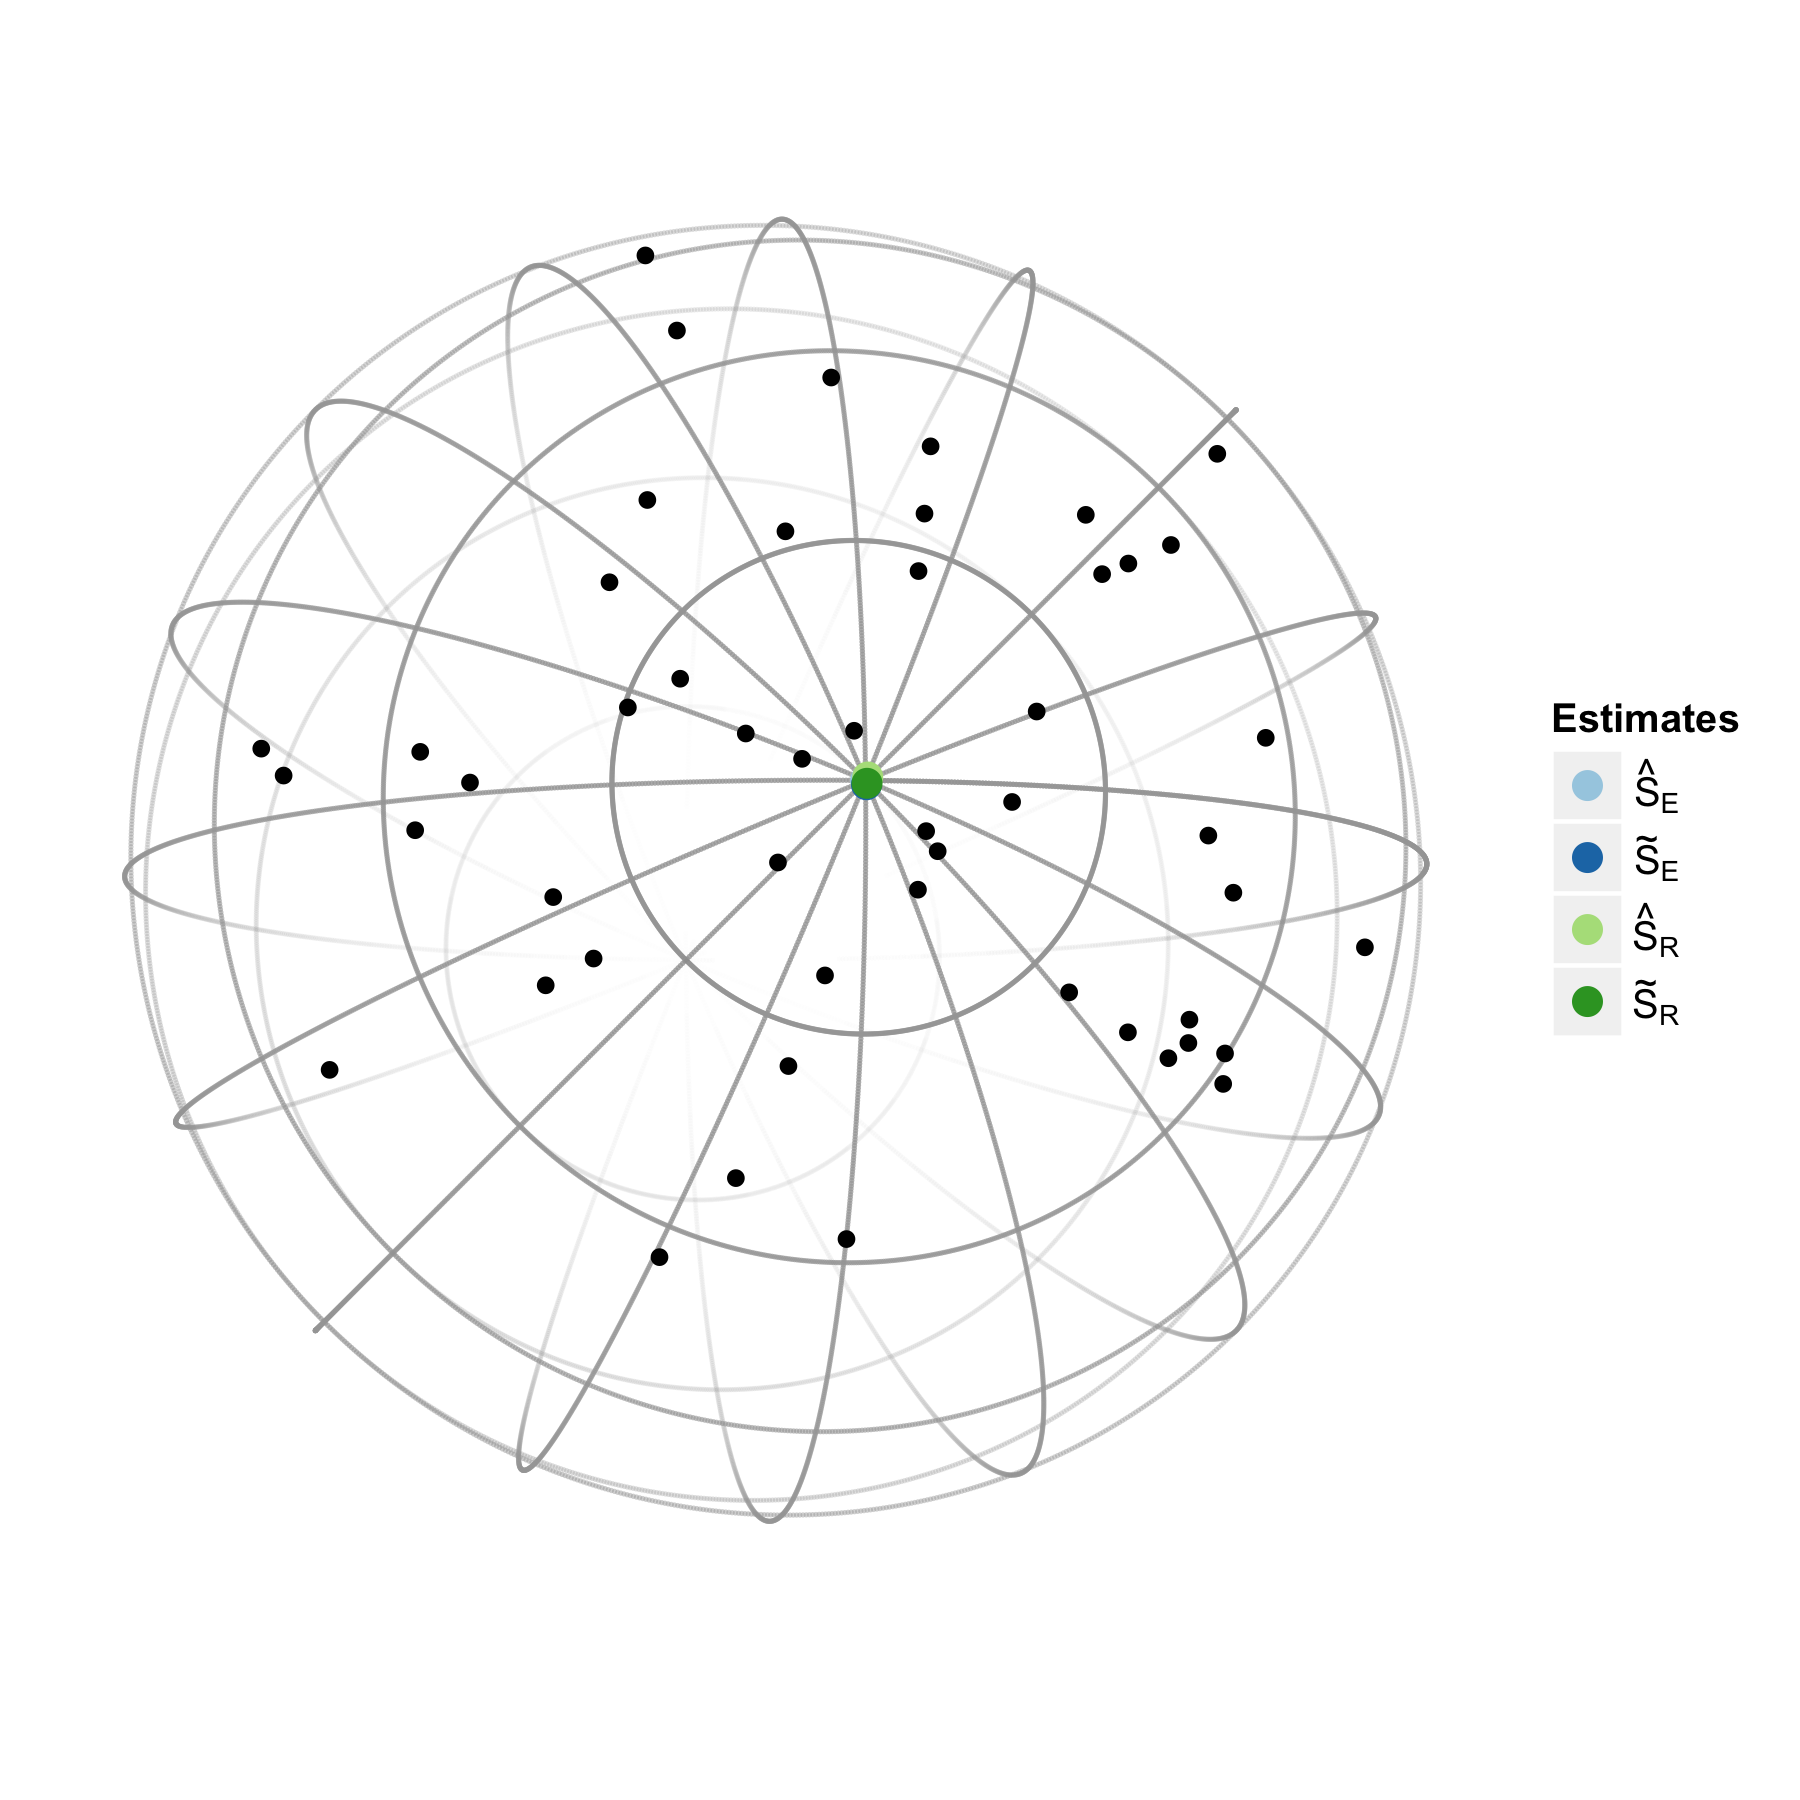
\includegraphics[width=\textwidth]{figures/eye2}\vspace{-1em}
		\caption{Point estimates}
		\label{fig:ests}
	\end{subfigure}
	\begin{subfigure}[h]{.25\textheight}
		\centering
		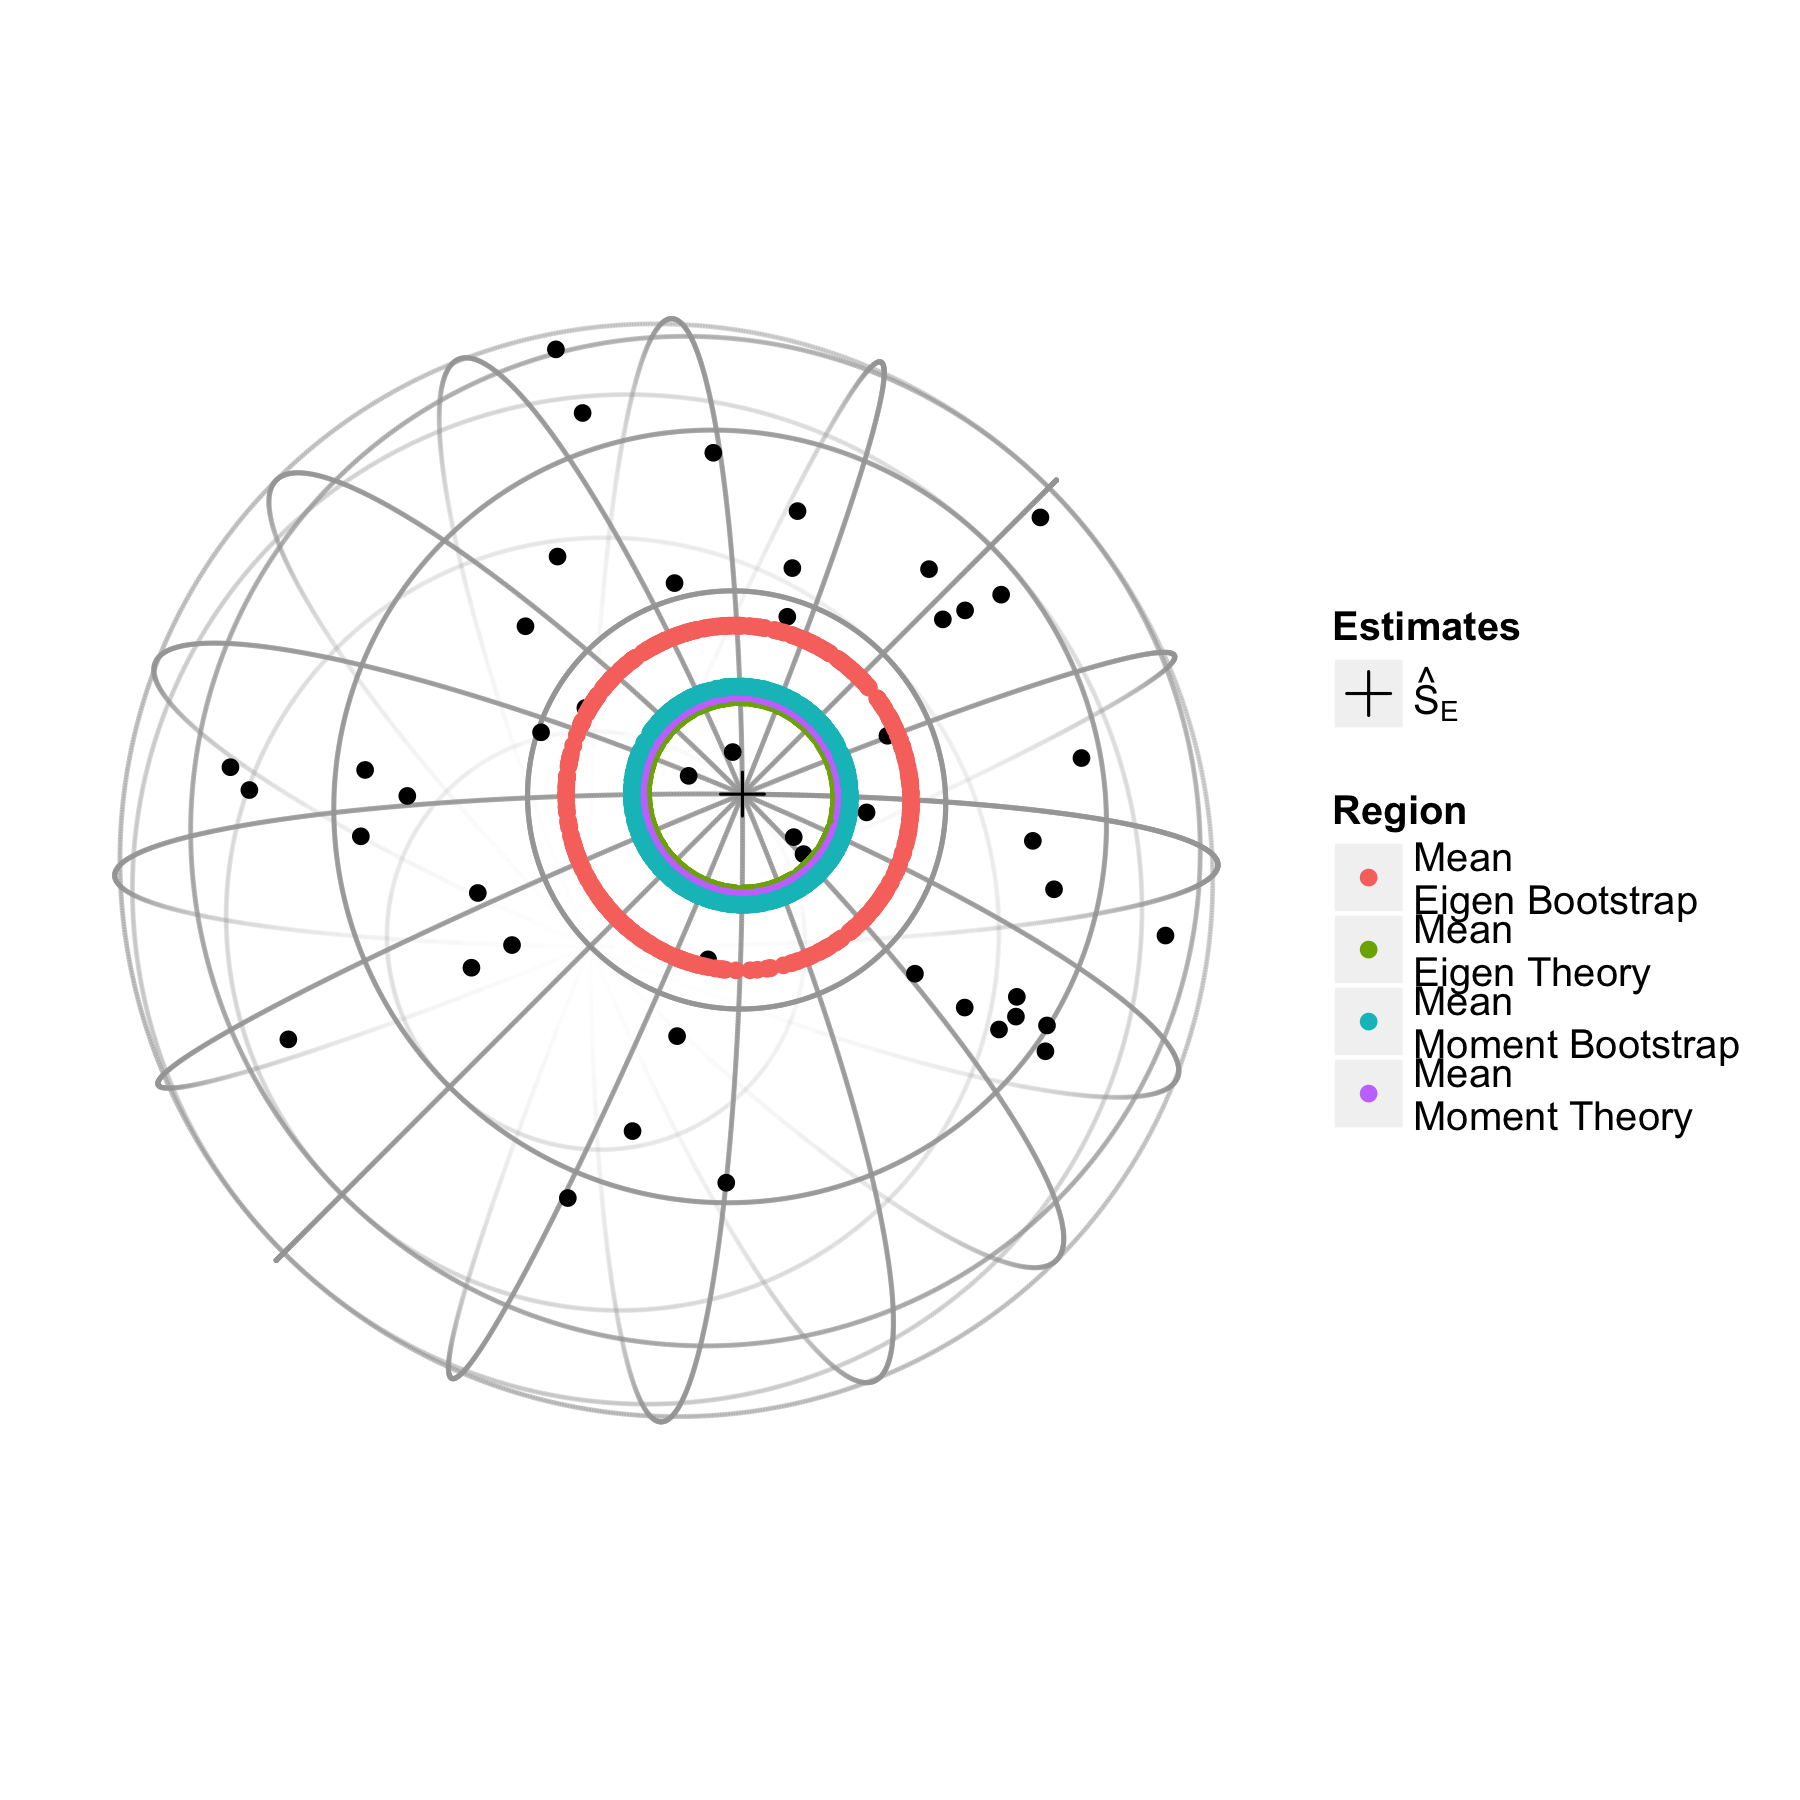
\includegraphics[width=\textwidth]{figures/eye3}\vspace{-1em}
		\caption{Confidence region estimates}
		\label{fig:regs}
	\end{subfigure}
	\caption{\label{figure:eye1}The $x$-axis of a random sample from the Cayley-UARS distribution with $\kappa=1$, $n=50$.  All for point estimates are displayed in (a) and all three region methods along with the projected mean are in (b).}
\end{figure}


\section{Datasets}

Datasets \code{drill} and \code{nickel} are included in the \pkg{rotations} package to illustrate how the two representations of orientation data discussed here are used in practice.  The \code{drill} dataset was collected to assess variation in human movement while performing a task \citep{rancourt1995}.  Eight subjects drilled into a metal plate while being monitored by infared cameras. Quaternions are used to represent the orientation of each subjects' wrist, elbow and shoulder in one of six positions.  For some subjects several replicates are available.  See \cite{rancourt2000} for one approach to analyzing these data.

In the \code{nickel} dataset rotation matrices are used to represent the orientation of cubic crystals on the surface of a nickel sample measured with Electron Backscatter Diffraction.  Each location on the surface of the nickel is identified by the \code{xpos} and \code{ypos} columns while the \code{rep} column identifies which of the fourteen replicate scans that measurement corresponds to.  The last nine columns, denoted \code{v1}-\code{v9}, represent the elements of the rotation matrix at that location in vector form.  See \cite{bingham2009, bingham2010b, stanfill2013} for more details. In the example code below we illustrate how to load the datasets into an R session and some basic analysis techniques.  For the \code{drill} dataset we estimate the central orientation of the readings for Subject 1's wrist.  For simplicity we round to three digits.

\begin{example}
> data(drill)
> head(drill)
  Subject Joint Position Replicate    Q1     Q2      Q3    Q4
1       1 Wrist        1         1 0.944 -0.192 -0.156 0.217
2       1 Wrist        1         2 0.974 -0.120 -0.111 0.158
3       1 Wrist        1         3 0.965 -0.133 -0.141 0.177
4       1 Wrist        1         4 0.956 -0.134 -0.115 0.233
5       1 Wrist        1         5 0.953 -0.199 -0.061 0.222
6       1 Wrist        2         1 0.963 -0.159 -0.127 0.177
> Subj1Wrist<-subset(drill, Subject == '1' & Joint == 'Wrist')
> data <- as.Q4(Subj1Wrist[,5:8])
> mean(data)
0.987 - 0.070 * i - 0.134 * j + 0.049 * k
>
> data(nickel)
> head(nickel[,1:6])
  xpos  ypos rep     v1     v2      v3
1  0.0 0.346   1 -0.648 -0.727 -0.879
2  0.2 0.346   1  0.686 -0.647  0.371
3  0.4 0.346   1 -0.330  0.685  0.716
4  0.6 0.346   1 -0.289 -0.336 -0.052
5  0.8 0.346   1 -0.623  0.708 -0.697
6  1.0 0.346   1 -0.727  0.375  0.642
\end{example}

\section{Summary}

In this manuscript we introduced the \pkg{rotations} package and demonstrated how it can be used to generate, analyze and visualize rotation data.  It is compatible with the quaternion specific \pkg{onion} package by applying its \code{as.quaternion} function to a transposed \code{"Q4"} object.  This gives the user access to a wide range of algebraic functions unique to quaternions.  Due to differences in data representations, the \pkg{orientlib} package is not immediately compatible with our package but a connection is possible.  Bridging the gap between these two packages would give the \pkg{orientlib} users access to data analysis methods for two Euler angle representations.  Computational speed of the \pkg{rotations} package has been enhanced through use of the  \CRANpkg{Rcpp} and \CRANpkg{RcppArmadillo} packages \citep*{eddelbuettel2013,eddelbuettel2013b}.  In addition the algorithms implemented in the \pkg{rotations} package are the fastest presently available, more so than competing algorithms of \cite{hartley2013}.  In future version of the package we plan to extend the parameterization and estimator sections to include robust estimators currently being developed by the authors.  

\bibliography{stanfill-hofmann-genschel}

\address{Bryan Stanfill\\
  Department of Statistics\\
  Iowa State University\\
  Ames, IA 50011}\\
\email{stanfill@iastate.edu}

\address{Heike Hofmann\\
  Department of Statistics\\
  Iowa State University\\
  Ames, IA 50011}\\
\email{hofmann@mail.iastate.edu}

\address{Ulrike Genschel\\
  Department of Statistics\\
  Iowa State University\\
  Ames, IA 50011}\\
\email{ulrike@mail.iastate.edu}

